\newpage
\section{Symmetric abstractions}\label{symmstric-abstractions}


% Reasonably well understood how symmetric abstractions can improve computational complexity.
% But, want to understand how they effect sample complexity.

% symmetry is cool
Symmetry is a concept from pure mathematics, which has found major success in physics, ...
(why has it found such success in physics? beauty, compression, ... Occam's razor)
But what do we mean by symmetry?

% example


% occam's razor
Occam's razor is a core idea behind much of statistics, ML and science. Simple
hypotheses should be preferred as the are more likely to be right. This intuition
can be viewed a little more formally through a Bayesian perspective.

% symmetry and occams razor
How does symmetry relate to simplicity?

% how can symmetry help? more concretely
But, why do we care about symmetry?
\begin{displayquote}
We want the ability to identify symmetries in state-actions-rewards (/values) and use that knowledge to share rewards (/values) between 'similar' state-actions.
\end{displayquote}
It gives us a way to find 'simple' hypotheses that fit the data.
Imagine we knew that a learning problem was symmetry in some sense, for example ...
How might we exploit this knowledge to learner more efficiently?
Reduce variance, generalise in more 'intelligent' ways.

% but. discovery
But.

% relation to abstraction
???

% related work on complexity / occam's razor
This ability is currently lacking in the ML tool kit. There has been much work done
to

%  why do we care?
For sample efficiency!! Inductive bias. Generalise in the right way without making observations.

\subsubsection{Definition}

?!?!
The most useful starting point. Finite groups.

A group is a set, $G$, together with an operation $\circ$ (called the group law
of $G$) that combines any two elements $a$ and $b$ to form another element.
To qualify as a group, the set and operation, $(G, \circ)$, must satisfy four requirements known as the group axioms:

\begin{itemize}
	\tightlist
	\item \textbf{Closure:} For all $a, b \in G$, the result of the operation $a \circ b$ is also in $G$.
	\item \textbf{Associativity:} For all $a,b,c \in G$, $(a\circ b) \circ c = a\circ (b\circ c)$.
	\item \textbf{Identity element:} There exists and element $e\in G$ such that, for every element $a\in G$, the equation $e\circ a = a\circ e = a$ holds.
	\item \textbf{Inverse element:} For each $a \in G$, there exists an element $b \in G$, commonly denoted $a^{−1}$, such that $a \circ b = b \circ a = e$.
\end{itemize}

\subsection{Symmetries for RL}\label{mdp-homomorphism}

Which types of symmetry can exist in RL problems?
% How hard is it to find these symmetries?
% Are some harder than others?

\begin{figure}[h!]
	\centering
	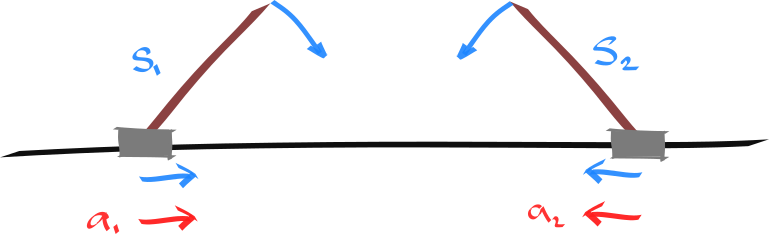
\includegraphics[width=1\textwidth,height=0.25\textheight]{../../pictures/drawings/cart-pole-mirror.png}
	\caption{Two mirror symmetric states of a cart pole.}
\end{figure}

% Need to show this is actually a symmetry, isomorphic to $S_2$?!?

These two objects are symmetric about a mirror plane (Need to draw).
Symmetric because there exists $f$ such that ...

% Want symmetry for efficient exploration / sample efficiency. !!!!
% Rather than picking actions; randomly, to minimise uncertainty, to ...?
% We want to pick actions to help us identify symmetries in the MDP.
% How does this help us increase the sample efficiency?
%
% If we are using something like neural counts. How does it generalise it density estimates!?
% Want symmetries!!!

\vspace{5mm}

As pointed out in \ref{abstraction}, the notion of an abstraction is captured by a homomorphism.
So, what would it look like if we had a MDP homomorphism?

What does it preserve?!?!

\cite{Ravindran2002}

$\mathcal H: \mathcal M\to \mathcal M$.

\begin{align}
P(f(s')|f(s), g_s(a)) = \sum_{s''\in [s']_f} P(s''| a, s) \\
r(f(s), g_s(a)) = r(s, a)
\end{align}


To be done.

\begin{itemize}
\tightlist
  \item temporal symmetries
  \item approximate symmetries (algorithm and complexity)
  \item inference of symmetries under uncertainty (algorithm and complexity)
  \item complexity measure / inductive bias
\end{itemize}

\subsection{Exploitation}

\begin{displayquote}
\textit{Once have discovered a symmetry, how might we exploit that knowledge?}
\end{displayquote}

\subsubsection{Exploiting symmetry for efficient control}

% Simple and well demonstrated.

Model minimisation. (are there any alternatives?)

...\cite{NARAYANAMURTHY}

\subsubsection{Exploiting symmetry for efficient inference}

\cite{Chen2019}
\ref{symmetry-inference}

\subsubsection{Exploiting symmetry for efficient exploration}

\cite{Holtzen2019}

Want to demonstrate this.
{\color{red}TODO max ent + abstraction experiments}

\subsection{Discovery}

% This is about generalising using an inductive bias towards symmetry.

Symmetry is a stricter notion of similarity. How can it be discovered?

Relationship to disentanglement. \cite{Higgins2018} which makes a lot of sense because ...

Connection to causal hierarchy. Cite Pearl. Association, intervention, counterfactuals.
Also recently noted by \cite{Caselles-Dupre2019}, ... where they assume that
the group actions are the actions of the RL environment.
This doesn't really make sense. Also, will miss many symmetries like ???

A couple parts. Discovery of symmetries, exploration of the knowledge of symmetries.

Unsupervised discovery. Not much success yet. Only when using some kind of supervised signal.

\cite{Ho2019a, Lim2019, Cubuk2018, Cubuk2019}
Discover which symmetries apply to a given domain, and at what magnitude.
The optimisation problem becomes one of picking the probability of each op and its magnitude.
There is a small set of ops (aka symmetries) that are given:
\textit{Identity, AutoContrast, Equalize, Rotate, Solarize, Color, Posterize, Contrast,
	Brightness, Sharpness, ShearX, ShearY, TranslateX, TranslateY.}
Uses validation error as a reward for learning.


\subsubsection{Inferring symmetries from experience}

% How easy is it to solve this symmetry inference problem?

% HOW?!

What does this buy us? If have sufficient data to tell us that $x$ and $y$ are
similar, say that they are mirror images of each other.
As an unsupervised pre-training step. Then apply and share labels and learn more quickly?
What else can $x$ tell us about $y$?

\cite{Yang2019}

Or end to end? As we get more certain that x and y are similar, we more strongly
encourage their symmetry through one of the methods outlined above.
Is it possible (/easier) to learn that x and y are similar (in terms of their labels) before (accurately) learning their labels.



Want to have an inductive bias towards simpler symmetries. But, how can we do this without needing to represent all possible symmetries?
A solution rejection sampling??


%
% - What about symmetries that are products of subgroups? $S = Z_2 \times Z_3$?
% Are they easier to infer?
% - Within the same $n$. Is there a notion of more or less complex group structures??
% - Need to show that NNs dont have the right symmetric inductive bias. They dont generalise. !!!

% Examples

% - Knowing that; range $= [0,360)$, and $0, 45, 90, 135, 180$, all are similar. I guess that we are in cyclic group $8$ and therefore $225, 270, 315$ are also similar. Key is that I know that $0, 45, 90, 135, 180$ are related by $0+0, 0+45, 0+45+45, 0+45+45+45, 0+45+45+45+45$.
% - Cart pole. $V^{\pi(s, a)}(s') = V^{\pi(-s, -a)}(-s') \forall s'$.


\subsubsection{Invariants}

Symmetries can be uniquely characterised by their invariants \cite{PeterOlver1999}.
What are the interesting invariants of MDPs? And how do they ???
But, what does this symmetry imply about other quantities of interest for RL?

Invariance, $f(g(x)) = f(x)$, equivariance, $f(g(x)) = g(f(x))$.

In general we want to know;

\begin{itemize}
	\tightlist
	\item We have $n$ different 'symmetries'. But are they really different?
	\item Which symmetries share some invariants?
	\item Which invariants uniquely characterise this symmetry?
\end{itemize}

With this knowledge, we could identify symmetries via their invariants!?!
We can observe invariant properties. (not clear to me how you observe a symmetry!?)

We briefly explore this in \ref{game-invariants}.


\subsection{Inductive bias towards seeing symmetry}

% WANT GENERALISATION!

The problem is the cost of inferring symmetry

Guess that things are symmetrc, despite observing they are not.

\begin{align}
P(\tau, r| \theta)
\end{align}

Clip to nearest symmetric abstraction.

Have a prior belief that MDPs are sampled from $M \sim ???$.

\subsubsection{Langevin dynamics}

\begin{align}
\mathop{\text{argmin}}_{\theta} D(\bar \theta, \theta)
\end{align}

Where $\bar \theta$ is the nearest symmetric set of parameters.

\begin{align}
\theta = \theta_t - \eta \nabla_\theta \mathcal S(\theta) + w
\end{align}

Langevin dynamics. Where $w$ is sampled from some noise distribution.
Therefore, we get a distribution over $\theta$.
Only do a few iterations, so we sample $\theta$ that are near by!?!?
The $\nabla_\theta \mathcal S(\theta)$ pulls us towards symmetric parameters.

Need a differentiable measure of symmetry.!?
If I actually find this, we can just use it as a regulariser..!?!?!?


\subsubsection{Thompson sampling} \label{thompson-sampling}

{\color{red}TODO need to introduce this framework}

SARSA plus thompson sampling. Does this really work? Want to test.

\begin{algorithm}
	\caption{Thompson sampling}
	\begin{algorithmic}[1]

		\Procedure{TS}{$\gamma$}
		\State $\pi_t \sim \mathcal U(\Pi)$
		\While{not converged}
		\State $\tilde P, \tilde r \sim P_{\theta}(\cdot)$
		\State $Q_{t+1} =  r + \gamma P Q_t$ \Comment{Bellman operator}
		\State $\theta = \nabla_{\theta} P_{\theta}(P, r)$ \Comment{Max likelihood}

		\EndWhile
		\State \algorithmicreturn{ $\pi$}
		\EndProcedure

	\end{algorithmic}
\end{algorithm}

The way we parameterise the distribution over possible models (/ MDPs), $\theta$, has implicit inductive biases about the true structure of the model.
A way to add explicit inductive biases is via importance (/ rejection) sampling.

We can encourage the model to be more symmetric!?
How much computation does this cost?

But. How can we construct the distribution? We want to be able to take samples
from it.

Ok. Great we have this inductive bias. But it doesnt help exploration in the way I want it to...
The parameters we have learned are close to being symmetric in some way. So the complexity measure alters the likelihoods and makes the symmetric version the most probable.
How does this help exploration? More likely to sample the true model / a symmetric one. Need to be able to exploit this symmetry.

This solves the efficient inference problem. Not efficient exploration... How can we get both?
Sample an abstraction then lift it to the original MDP?!


Thompson sampling from estimates of similarity / symmetry.
\begin{enumerate}
	\tightlist
	\item Keep estimate of similarity. $\chi(x_i, x_j)_{t+1} = \chi(x_i, x_j)_t + ?$
	\item Construct distribution over likely abstractions $P(x_i = x_j) \propto e^{\chi(x_i, x_j)_t}$. $\mathcal F = P(f|\chi_t)$
	\item Sample an abstraction. $f\sim \mathcal F$
	\item Reduce the MDP $M' = f(M)$
\end{enumerate}


For now just assume we have an accurate estimate of the model.
What does acting optimally wrt the reduced model mean for exploration and convergence??


% How to reason about the tradeoff between symmetry and fitting the data!?.
